\clearpage
\section{Bifurcations}
\begin{colbox}
	For each of the following systems, identify which types of bifurcation occur at a critical \(r\): saddle node, transcritical, or pitchfork. Determine the critical \(r\) values and sketch the bifurcation diagram \(x^*\) vs.\ \(r\). Draw the flow on the phase line before and after the bifurcation.
	\begin{itemize}
		\item \(\dot{x}=1+rx+x^2\)
		\item \(\dot{x}=-x+\frac{rx}{1+x^2}\)
		\item \(\dot{x}=x\ins{r-e^x}\)
		\item \(\dot{x}=r-\cosh x\)
	\end{itemize}
\end{colbox}
\subsection{\(\dot{x}=1+rx+x^2\)}
We can find the roots of the right hand side by
\begin{equation}
	x^* = \frac{-r\pm\sqrt{r^2-4}}{2}=\frac{-r\pm\sqrt{\ins{r+2}\ins{r-2}}}{2}
\end{equation}
We can see that there are either no critical points (when \(-2<r<2\)), one critical point (at \(r=\pm2\)) or two critical points (when \(\abs{r}>2\)). Therefore both \(r=\pm2\) are saddle node bifurcations. 
\begin{figure}[!htb]
	\begin{center}
		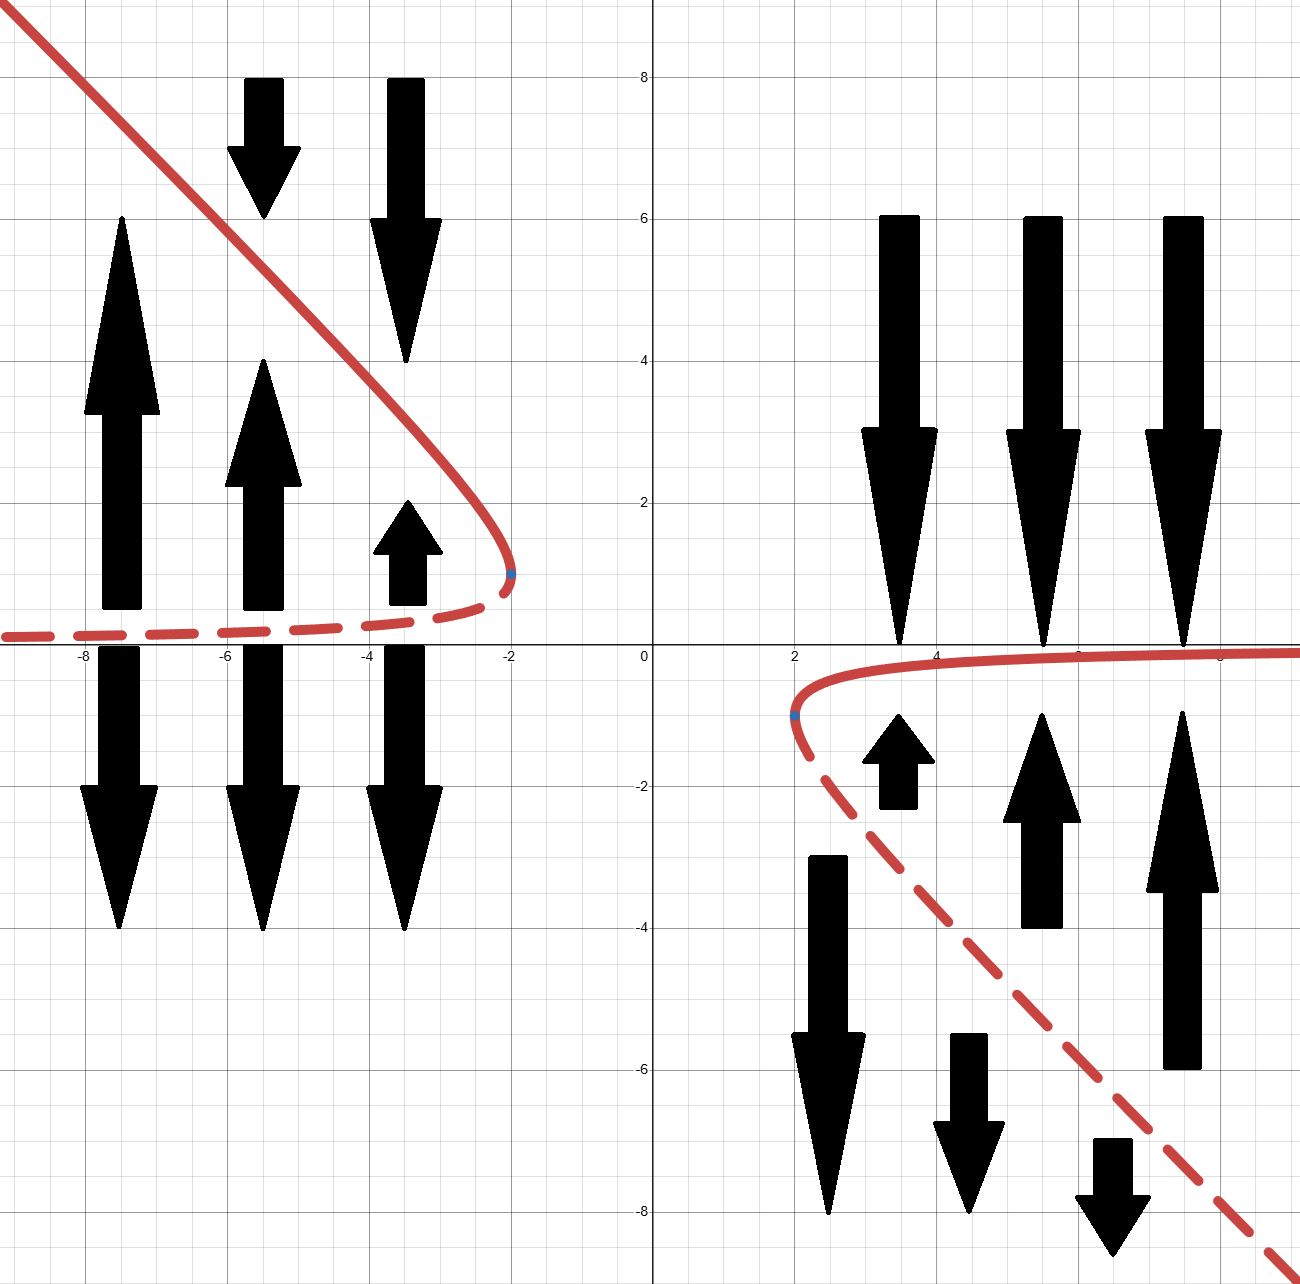
\includegraphics[width=0.5\textwidth]{bifuraction1.png}
	\end{center}
\end{figure}
\subsection{\(\dot{x}=-x+\frac{rx}{1+x^2}\)}
Simplifying the right hand side
\begin{equation}
	-x+\frac{rx}{1+x^2} = x\ins{\frac{r}{1+x^2}-1}
\end{equation}
threfore the critical points are at 
\begin{align}
	x=0 && x = \sqrt{r-1}
\end{align}
Therefore there is always a critical point at \(x=0\) but also another one which moves with \(r\) and appears when \(r\ge1\). Looking at the derivative of the right hand side at \(x=0\)
\begin{equation}
	f'(0) = -1 + \left.\frac{r\ins{1+x^2}-2rx^2}{\ins{1+x^2}^2}\right|_{x=0}=r-1
\end{equation}
Therefore the critical point at \(x=0\) changes its stability depending on the value of r, therefore this is a transcritical bifurcation. As for the other point
\begin{equation}
	f'(\sqrt{r-1}) = -1 + \left.\frac{r\ins{1+x^2}-2rx^2}{\ins{1+x^2}^2}\right|_{x=\sqrt{r-1}}= \frac{2r\ins{r-1}}{r^2} = 2\ins{1-\frac{1}{r}}
\end{equation}
Which is always positive for \(r\ge1\), so it is unstable.
\begin{figure}[!htb]
	\begin{center}
		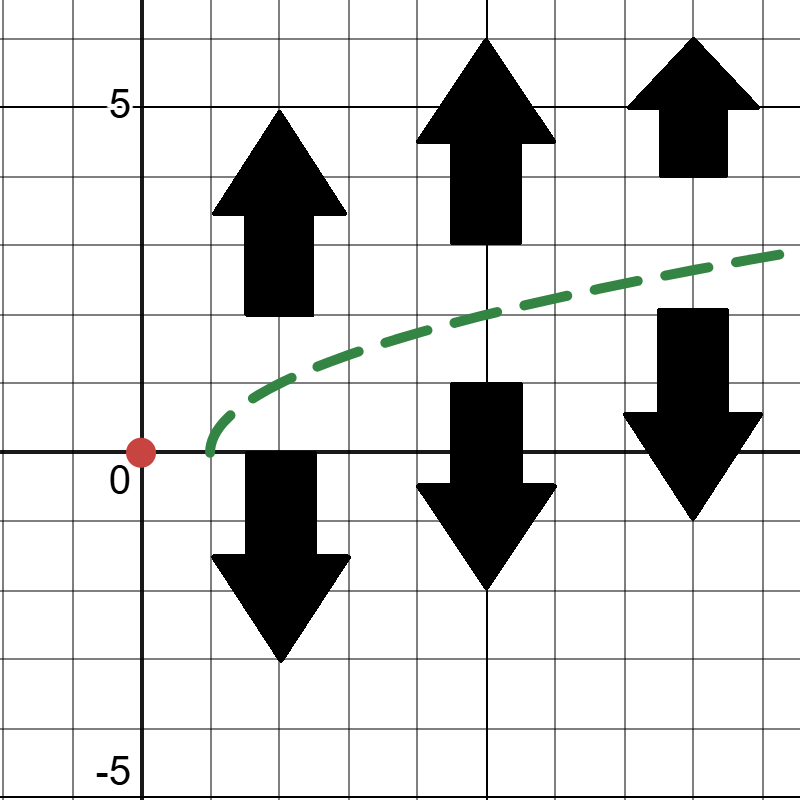
\includegraphics[width=0.5\textwidth]{bifurcation2.png}
	\end{center}
\end{figure}
\newpage
\subsection{\(\dot{x}=x\ins{r-e^x}\)}
It's easy to see the critical points are \(x=0,\ln{r}\). The derivative is
\begin{equation}
	f'(x) = r-e^x-xe^x = r-e^x\ins{1+x}
\end{equation}
therefore
\begin{align}
	f'(0) = r-1 && f'(\ln{r}) = -r\ln r
\end{align}
The critical point at \(x=0\) changes its stability, and the critical point at \(x=\ln r\) is always stable. Therefore this is a transcritical bifurcation.
\begin{figure}[!htb]
	\begin{center}
		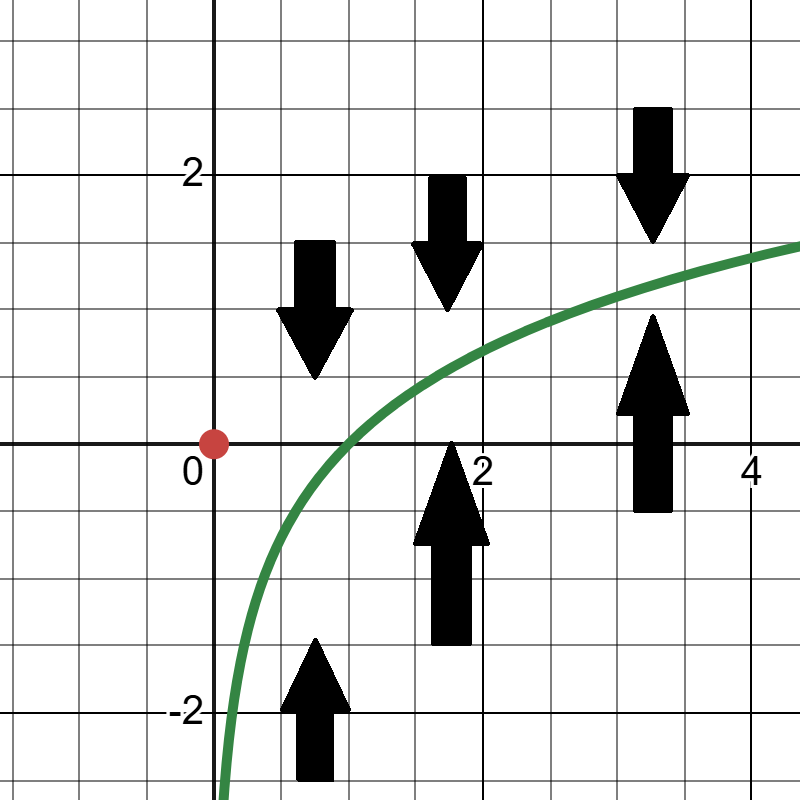
\includegraphics[width=0.5\textwidth]{bifurcation3.png}
	\end{center}
\end{figure}
\newpage
\subsection{\(\dot{x}=r-\cosh x\)}
The root of the right hand side is, expectedly, \(x=\cosh^{-1}(r)\). The derivative is \(f'(x) = -\sinh x\). Therefore the derivative at the critical point is
\begin{equation}
	f'(\cosh^{-1}(r)) = -\sinh(\cosh^{-1}(r)) \le 0 \quad \text{(thanks desmos)}
\end{equation}
So the critical point is always stable. This is also a transcritical bifurcation.
\begin{figure}[!htb]
	\begin{center}
		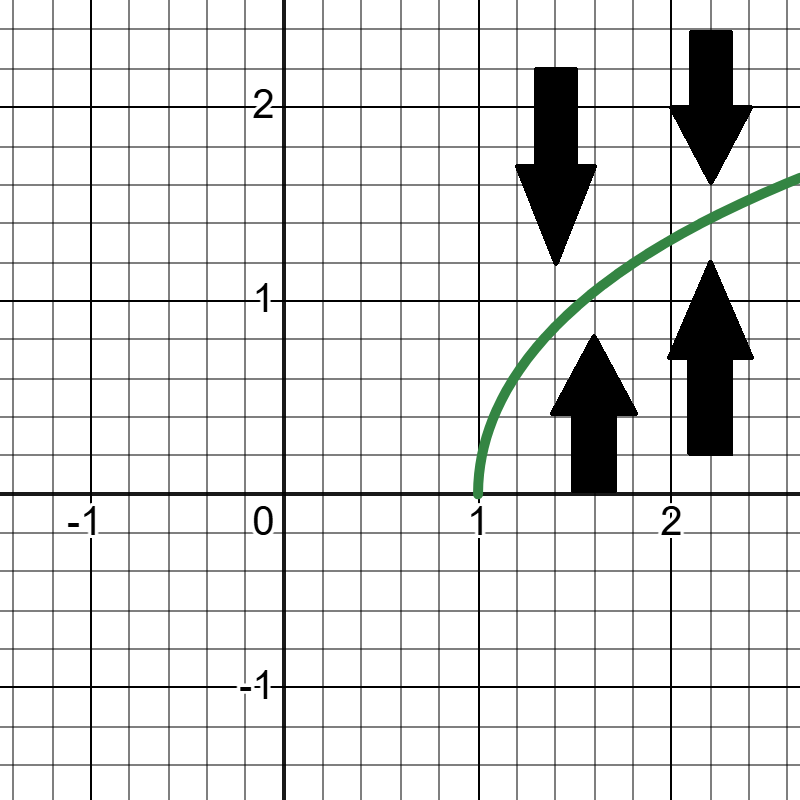
\includegraphics[width=0.5\textwidth]{bifurcation4.png}
	\end{center}
\end{figure}